\chapter{Experiments}
\label{chap:4}

- BO : We set the initial sample count $M = 10$ and the iteration count $N = 200$.

\section{Implementation}

\subsection{Problem environment}
In early test runs we used \texttt{MATLAB} implementations of cart pole, acrobot, and mountain car adapted from \cite{joseCode}. But later we implemented the OpenAI Gym to have a wide range of problem environments available and to have consistent rewarding functions. Otherwise, the rewarding function would depend on the source and therefore produce less comparable results.






\subsection{Action selection}

In continuous action space we use a linear policy to action mapping

$$a = f_s(s)^\top x + \epsilon_a,$$

with a small gaussian noise $\epsilon_a$ needed for stochastic policies. So the actions are Gaussian distributed:

$$a \sim \mathcal{N}(f_s(s) x,\epsilon_a^2).$$

In discrete action space environments we use a parametric soft-max action selection policy:

$$P(a|s)= \frac{\exp(f_s(s)^\top x_a)}{\sum_{i\in A} \exp(f_s(s)^\top x_i)}.$$

Again it consists of the linear mapping $f_s(s)^\top x$, and $A$ holds all possible actions. The resulting action is then sampled from the probability of action $a$ given state $s$.

The state feature function $f_s(s)$ is defined for each environment.

\section{Cart pole}

\begin{wrapfigure}{R}{0.5\textwidth}
    \centering
    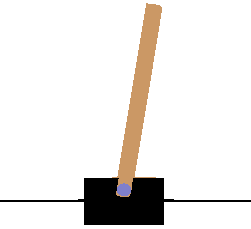
\includegraphics[width=0.45\textwidth]{/home/sebastian/Documents/bscThesis/img/cartpole.pdf}
    \caption{Visualization of the cart pole rendered by the Open AI Gym\label{fig:cartpolePygym}}
\end{wrapfigure}

The cart pole environment consist of a cart with a pole attached to its top. The cart is accelerated to the left or the right to balance the pole for as long as possible. An episode starts with small random state values and it ends when the maximum of time steps or a specifc state is reached. The state values contain the position and the velocity of the cart, and the angle and the angular velocity of the pole. Each of these four state values are set uniformly random between -0.05 and 0.05 at the beginning. The episode ends after 200 time steps or if the pole falls below 12 degrees relative to the vertical. It also ends when the cart is more than 2.4 meters away from the center. For each completed time step a reward of 1 is returned.

% \begin{figure}
%     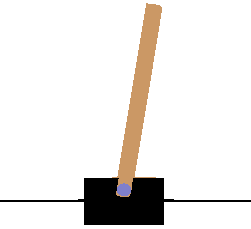
\includegraphics{/home/sebastian/Documents/bscThesis/img/cartpole.pdf}
%     \caption{Visualization of the cart pole from Open AI Gym\label{fig:cartpolePygym}}
% \end{figure}

The cart pole implementation from Open AI Gym (figure \ref{fig:cartpolePygym}) accepts a discrete action value for either applying force to the left (-1) or to the right (1). With the four state values and an additional bias value we have five dimensions for each discrete action resulting in a total of ten dimensions. In our own cart pole simulation we only use the four state parameters for calculating an continuous action value between -1 and 1. Therefore this policy has only four dimensions.


\section{Acrobot}

\begin{wrapfigure}{R}{0.25\textwidth}
    \centering
    
\includegraphics[width=0.20\textwidth]{/home/sebastian/Documents/bscThesis/img/acrobot.pdf}
    \caption{Visualization of the Acrobot rendered by the Open AI Gym\label{fig:acrobotPygym}}
\end{wrapfigure}

The acrobatic robot has two joints and two pendulums. The upper joint has a fixed position. It connects to the first pendulum, which is attached to the second joint. A torque can be applied to that second joint, which controls the second pendulum. The goal is to gain enough momentum and swing the end of the second pendulum above a certain mark. The angle between vertical and the first pendulum and the angle between the two pendulums form the six state parameters. Four parameters are the sine and the cosine of these two angles each, whereas the last two parameters are the angular velocities. The discrete action can has the values -1, 0 or 1. Each value stands for the amount of torque applied to the joint between the two pendulum links. With the six state values, an additional bias value, and three discrete action possibilities we get 21 dimensions for the Acrobot policy.

\section{Mountain car}

\begin{wrapfigure}{R}{0.4\textwidth}
    \centering
    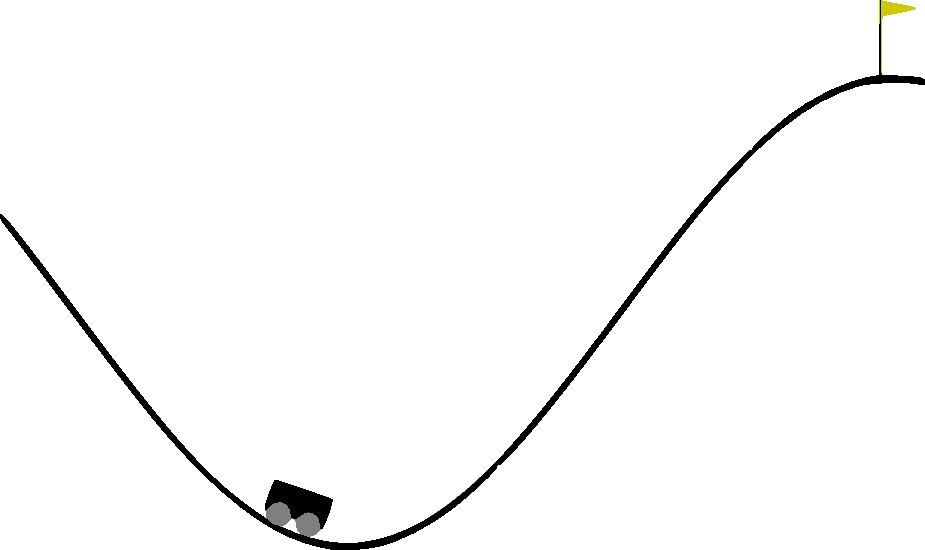
\includegraphics[width=0.35\textwidth]{/home/sebastian/Documents/bscThesis/img/mountaincar.pdf}
    \caption{Visualization of the mountain car rendered by the Open AI Gym\label{fig:mountaincarPygym}}
\end{wrapfigure}

In the mountain car task, an underpowered car tries to drive uphill. It can only reach the goal on the right side if it uses both hills to gain momentum. The end of the left hill is an inelastic wall, so if the car hits it, the velocity is set to zero.

%
% \begin{figure}
%     \begin{center}
%         \fbox{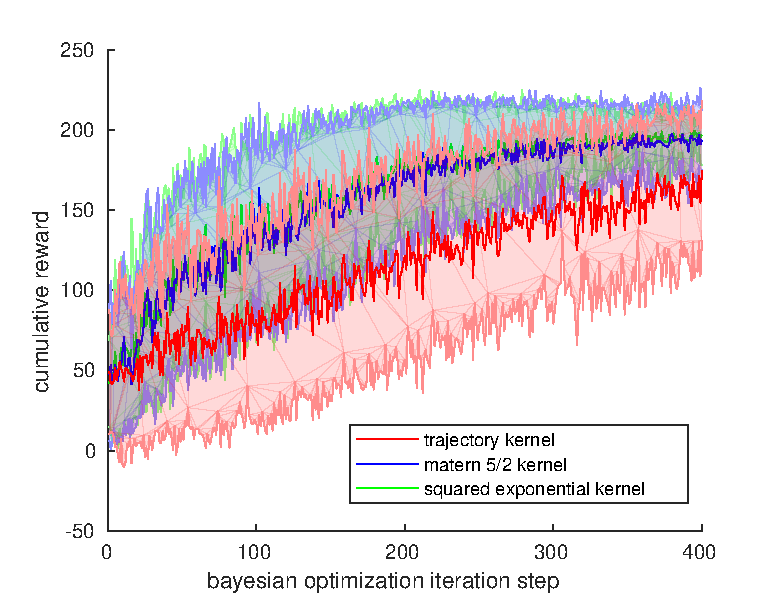
\includegraphics{/home/sebastian/Documents/bscThesis/img/cartpole_matlab_conti_newreward_local}}
%         \caption{Local opt, 4 dim. Mean and standard deviation from 32 trials of each kernel. Cartpole matlab implementation with new reward function, 200 timesteps, and continuous action selection.}
%     \end{center}
% \end{figure}
%
% \begin{figure}
%     \begin{center}
%         \fbox{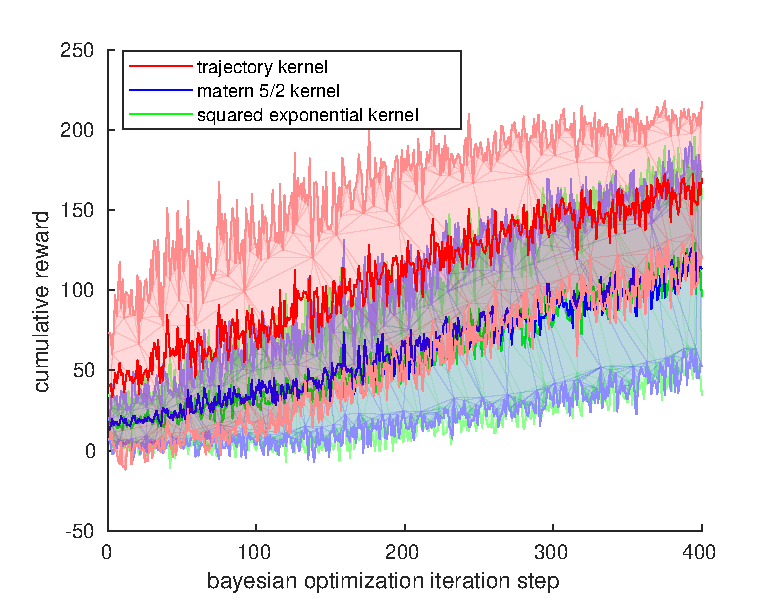
\includegraphics{/home/sebastian/Documents/bscThesis/img/cartpole_pygym_disc_local}}
%         \caption{Local opt, 10 dim. Mean and standard deviation from 32 trials of each kernel. Cartpole python gym implementation, 200 timesteps, and discrete action selection.}
%     \end{center}
% \end{figure}
